\documentclass{article}
\usepackage{amsmath}
\usepackage{MnSymbol}
\usepackage{wasysym}
\usepackage{graphicx}
\usepackage{float}
\usepackage{pdfpages}
\usepackage[numbered,framed]{matlab-prettifier}
\usepackage[export]{adjustbox}
\begin{document}
\begin{center}
\LARGE \bfseries{Answers to Problem Set 3}\\
 Group name: Ferienspass\vspace{.5cm}\\
 \normalsize \normalfont
  Sebastian K\"uhnl: 5642348\\
  Alexander D\"uck (as: reebyte): 5504077\\
  Patrick Blank (as: paddyblank): 6729110\\
  Christian Wierschem: 6729288
\end{center}
\normalsize	

\section{Question 1}
Newton Optimization Algorithm
 \lstinputlisting[style=Matlab-editor]{Newton_opt.m}
 The functions:
   \lstinputlisting[style=Matlab-editor]{f1.m}
  \lstinputlisting[style=Matlab-editor]{f2.m}
\section{Question 2}
\subsection{Subquestion 1}
From the slides, we get the following conditions for the variables on the balanced growth path
\begin{equation}
s_k f\left(k^*,h^*\right)-\left(\delta_k +g+n+ng\right)k^*=0  
\end{equation}
\begin{equation}
s_h f\left(k^*, h^*\right) - \left(\delta_h + g + n + ng\right)h^* = 0.
\end{equation}
solving for $k^*$ and $h^*$, respectively, gives
\begin{equation}
k^*= \frac{s_k f\left(k^*,h^*\right)}{\left(\delta_k +g+n+ng\right)}
\end{equation}
\begin{equation}
h^* = \frac{s_h f\left(k^*,h^*\right)}{\left(\delta_h +g+n+ng\right)}.
\end{equation}
However, since $f\left(k^*,h^*\right)$ depends on the variables that we try to solve for, this is not the final form yet.\\
Since we are assuming $F\left(K_t,H_t,A_tL_t\right) = K_t^\alpha H_t^\beta \left(A_tL_t\right)^{1-\alpha-\beta}$, we can further solve the expression
\begin{equation}
f \left( k^*,h^* \right) = \frac{F \left( K_t,H_t,A_t L_t\right )}{A_t L_t} = \frac{K_t^\alpha H_t^\beta \left(A_tL_t\right)^{1-\alpha-\beta}}{A_t L_t} = \left(\frac{K_t}{A_t L_t}\right)^\alpha \left(\frac{H_t}{A_t L_t}\right)^\beta.
\end{equation}
By definition of $k^*$ and $h^*$, this is gives
\begin{equation}
f\left(k^*,h^*\right) = k_t^\alpha h_t^\beta.
\end{equation}
Now, inserting this into $3$ and $4$
\begin{equation}
k^*= \frac{s_k k_t^\alpha h_t^\beta}{\left(\delta_k +g+n+ng\right)} \Leftrightarrow k^*= \left(\frac{s_k h_t^\beta}{\left(\delta_k +g+n+ng\right)}\right)^{\frac{1}{1-\alpha}}
\end{equation}
\begin{equation}
h^* = \frac{s_h k_t^\alpha h_t^\beta}{\left(\delta_h +g+n+ng\right)} \Leftrightarrow h^*= \left(\frac{s_h k_t^\alpha}{\left(\delta_h +g+n+ng\right)}\right)^{\frac{1}{1-\beta}}.
\end{equation}
It becomes evident, that $k^*$ and $h^*$ are a function of each other. However, we can simply substitute and then solve for the expression depending on parameters only
\begin{equation}
 k^*= \left(\frac{s_k \left(\left(\frac{s_h k_t^\alpha}{\left(\delta_h +g+n+ng\right)}\right)^{\frac{1}{1-\beta}}\right)^\beta}{\left(\delta_k +g+n+ng\right)}\right)^{\frac{1}{1-\alpha}} 
\end{equation}
\begin{equation}
 h^*= \left(\frac{s_h \left(\left(\frac{s_k h_t^\beta}{\left(\delta_k +g+n+ng\right)}\right)^{\frac{1}{1-\alpha}}\right)^\alpha}{\left(\delta_h +g+n+ng\right)}\right)^{\frac{1}{1-\beta}}.
\end{equation}
which can now be solved for the respective variable. For $k^*$:
\begin{center}
\begin{align*}
 k^*&= \left(\frac{s_k \left(s_h k_t^\alpha \right)^{\frac{ \beta}{1-\beta}}}{\left(\delta_h +g+n+ng\right)^{\frac{\beta}{1-\beta}}\left(\delta_k +g+n+ng\right)}\right)^{\frac{1}{1-\alpha}} \\
 &= \left(\frac{s_k s_h^{\frac{ \beta}{1-\beta}}}{\left(\delta_h +g+n+ng\right)^{\frac{\beta}{1-\beta}}\left(\delta_k +g+n+ng\right)}\right)^{\frac{1}{1-\alpha}} k_t^{\frac{\alpha \beta}{1-\beta - \alpha + \alpha \beta}} \\
  &= \left(\frac{s_k s_h^{\frac{ \beta}{1-\beta}}}{\left(\delta_h +g+n+ng\right)^{\frac{\beta}{1-\beta}}\left(\delta_k +g+n+ng\right)}\right)^{\frac{1-\beta- \alpha + \alpha \beta}{\left(1-\alpha\right)^2 +\alpha \beta -\beta}} 
  \end{align*}
\end{center}
For $h^*$:
\begin{center}
\begin{align*}
 h^*&= \left(\frac{s_h \left(s_k h_t^\beta\right)^{\frac{\alpha}{1-\alpha}}}{\left(\delta_k +g+n+ng\right)^{\frac{\alpha}{1-\alpha}}\left(\delta_h +g+n+ng\right)}\right)^{\frac{1}{1-\beta}} \\
 &= \left(\frac{s_h s_k^{\frac{\alpha}{1-\alpha}}}{\left(\delta_k +g+n+ng\right)^{\frac{\alpha}{1-\alpha}}\left(\delta_h +g+n+ng\right)}\right)^{\frac{1}{1-\beta}} h_t^{\frac{ \alpha \beta}{1-\beta-\alpha +\alpha \beta}}\\
 &= \left(\frac{s_h s_k^{\frac{\alpha}{1-\alpha}}}{\left(\delta_k +g+n+ng\right)^{\frac{\alpha}{1-\alpha}}\left(\delta_h +g+n+ng\right)}\right)^{\frac{1-\beta- \alpha + \alpha \beta}{\left(1-\beta \right)^2 +\alpha \beta -\alpha}}.
\end{align*}
\end{center}
Thus, the solution vector becomes
\begin{center}
 $ \begin{bmatrix}
  k^* \\ h^*
 \end{bmatrix}'$ 
 =
  $ \begin{bmatrix}
  \left(\frac{s_k s_h^{\frac{ \beta}{1-\beta}}}{\left(\delta_h +g+n+ng\right)^{\frac{\beta}{1-\beta}}\left(\delta_k +g+n+ng\right)}\right)^{\frac{1-\beta- \alpha + \alpha \beta}{\left(1-\alpha\right)^2 +\alpha \beta -\beta}}  \\ \left(\frac{s_h s_k^{\frac{\alpha}{1-\alpha}}}{\left(\delta_k +g+n+ng\right)^{\frac{\alpha}{1-\alpha}}\left(\delta_h +g+n+ng\right)}\right)^{\frac{1-\beta- \alpha + \alpha \beta}{\left(1-\beta \right)^2 +\alpha \beta -\alpha}}
 \end{bmatrix}'$ 
 \end{center}
 \setcounter{subsection}{5}
 \subsection{}
 All questions that lie between the first and this one are excluded from this document since they only involved programming exercises. \\ \\
 The path to be interpreted:
 \begin{figure}[H]
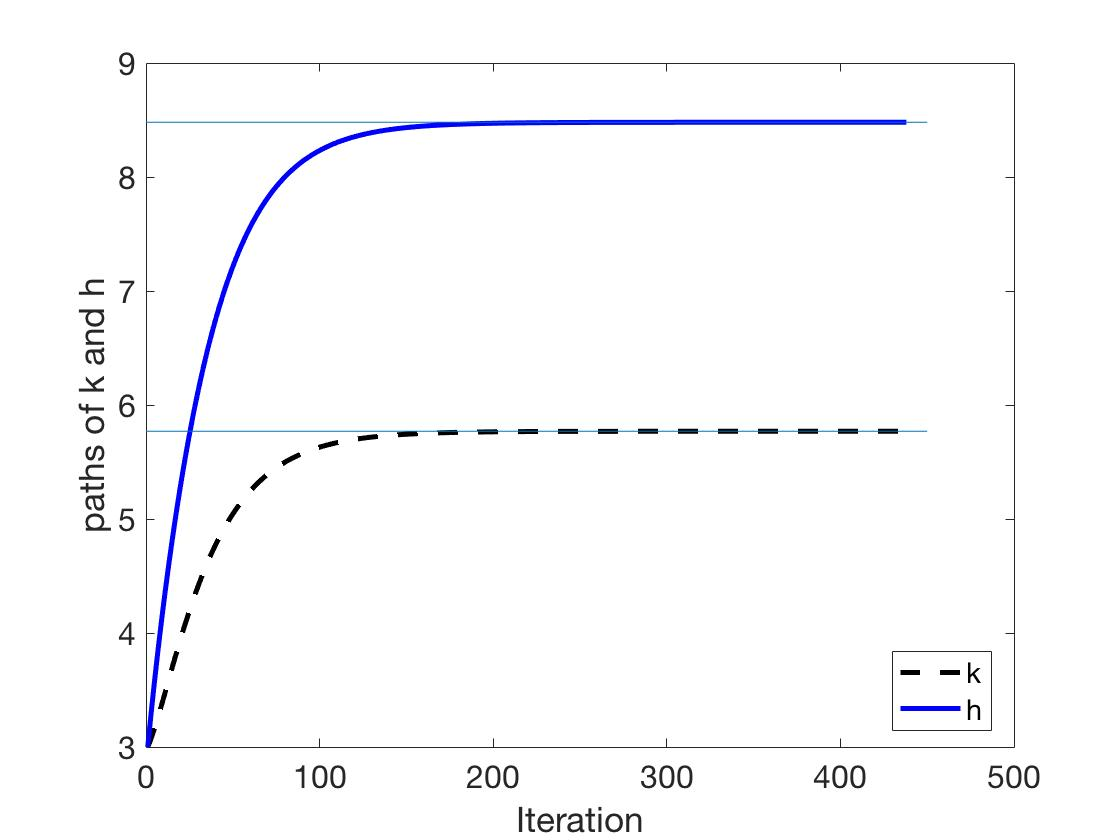
\includegraphics[width=\textwidth,height=\textheight,keepaspectratio, center]{Q2Sub6.jpg} 
\caption{Paths of $k^*$ and $h^*$}
\end{figure}
\noindent Both variables converge to the solution at the same time/speed. Optimal allocation human capital exceeds the optimal level of capital in all iterations.\\ A possible interpretation: That the balanced growth path level of human capital is greater than the balanced growth path level of physical capital could have two (simultaneous) reasons:
\begin{enumerate}
\item Human capital has a greater marginal product compared to physical capital
\item Human capital has a lower depreciation rate than physical capital
\end{enumerate}
The reasoning behind this it that if an additional unit of human capital yields more than an additional unit of physical capital, and lasts longer than it as well, and investment in human capital is preferred over an investment in physical capital. This goes on this way until a point is reached, where an investment in human capital has the same marginal-product-to-depreciation-rate as physical capital. The investment in the two goods will increase such that their levels always give the same marginal-product-to-depreciation-rate (which implies a constant ratio of human to physical capital (which can be seen in the graph as well)) until the entire income is spent. At this point, the balanced growth path level is reached.
\section{Question 3}
\section{Question 4}
%Given the constraints, the problem can be reformulated as
%\begin{equation}
%\max \sum_{t=0}^T \beta^t \frac{\left( a_t (1+r) + w_t -a_{t+1} \right )^{1-�\theta}-1}{1- \theta}
%\end{equation}
%which can then be stated as a Bellman equation, starting from the decision in period T
%\begin{equation}
%\nu_T = \max_{a_{T+1}} \left( \frac{\left( a_T (1+r) + w_T -a_{T+1} \right )^{1-�\theta}-1}{1- \theta} + \beta \times 0 \right)
%\end{equation}
%giving the policy function
%\begin{equation}
%a_{T+1} = 0
%\end{equation}
%which implies
%\begin{equation}
%\nu_T =   \frac{\left( a_T (1+r) + w_T  \right )^{1-�\theta}-1}{1- \theta}  .
%\end{equation}
%This result can now be used in the value function one period before the final period
%\begin{align}
%\nu_{T-1} &= \max_{a_{T}} \left( \frac{\left( a_{T-1} (1+r) + w_{T-1} -a_{T} \right )^{1-�\theta}-1}{1- \theta} + \beta  \nu_T  \right) \\
%&= \max_{a_{T}} \left( \frac{\left( a_{T-1} (1+r) + w_{T-1} -a_{T} \right )^{1-�\theta}-1}{1- \theta} + \beta \frac{\left( a_T (1+r) + w_T  \right )^{1-�\theta}-1}{1- \theta}  \right)
%\end{align}
%Maximizing wrt $a_T$:
%\begin{align}
%\frac{\partial \nu_{T-1}}{\partial a_{T}} = \left( a_{T-1} (1+r) + w_{T-1} -a_{T} \right )^{-�\theta} (-1) +  \beta \left( a_T (1+r) + w_T  \right )^{-�\theta} (1+r) = 0 \\
% \Leftrightarrow  \left( a_{T-1} (1+r) + w_{T-1} -a_{T} \right )^{-�\theta} =  \beta \left( a_T (1+r) + w_T  \right )^{-�\theta} (1+r) 
%\end{align}
\subsection{Analytical Solution}
From the Euler equation and the budget constraint we get that
\begin{align}
c_t &=\left( \beta (1+r) \right)^{- \frac{1}{\theta}} c_{t+1} \\
\sum c_t \left(  \frac{1}{1+r} \right)^{t} &= \sum w_t \left(  \frac{1}{1+r} \right)^{t} + a_0
\end{align}
Since we can express all $c_t$ as a function of $c_0$, we can write
\begin{align}
c_0 \sum \left(  \beta^{- \frac{1}{\theta}} (1+r)^{ \frac{\theta - 1}{\theta}} \right)^{t} &= \sum w_t \left(  \frac{1}{1+r} \right)^{t} + a_0
\end{align}
which allows to compute all $c_t$ after solving for $c_0$
\begin{align}
c_0 &= \frac{\sum w_t \left(  \frac{1}{1+r} \right)^{t} + a_0}{\sum \left(  \beta^{- \frac{1}{\theta}} (1+r)^{ \frac{\theta - 1}{\theta}} \right)^{t}} \\
c_{t+1} &= c_t \left( \beta (1+r) \right)^{ \frac{1}{\theta}}.  \\
\end{align}
This can now be implemented into an algorithm by using a for-loop.
\subsection{Algorithm}
\begin{lstlisting}[style=Matlab-editor]
%PS3 Problem 4
%No T is given, so declare it at the beginning of the program, and for any
%theta
clear;
close all;
clc;
T=20;
theta=1;
%variable initialization (fixed)
time=linspace(0,T,T+1); %just for plot
w=zeros(T+1,1);
w(1)=10;
beta=0.99;
r=0.05;
%these variables will be determined
a=zeros(T+1,1);
c=zeros(T+1,1);
%computation (could also be written as a function)
num=zeros(T+1,1);
denom=zeros(T+1,1);
if theta==1
    factor=beta*(1+r);
else
    factor=(1+r)^((1-theta)/theta)*beta^(1/theta);
end
for i=0:T
  num(i+1)=w(i+1)*(1+r)^(-i);  
  denom(i+1)=(factor)^i;  
end
c(1)=sum(num)/sum(denom);
for i=1:T
  a(i+1)=a(i)*(1+r)+w(i)-c(i);
  c(i+1)=c(i)*(beta*(1+r))^(1/theta); 
end
figure
plot(time,c,time,w,time,a);
legend('C','W','A')
acheck=a(end);
ccheck=c(end);
if (round(ccheck*1000)/1000==round(acheck*(1+r)*1000)/1000)
    display('True --> a_{T+1}= 0')
elseif (round(ccheck*1000)/1000>round(acheck*(1+r)*1000)/1000)
  display('a_{T+1}<0')
  disc=a(end);
  subst=zeros(T+1,1);
  for i=0:T
    subst(i+1)=(1+r)^i*((beta*(1+r))^(i/theta))^T-i;  
  end
  d=sum(subst);
  c(1)=c(1)-d;
  for i=1:T
    c(i+1)=c(i)*(beta*(1+r))^(i/theta);  
    a(i+1)=a(i)*(1+r)+w(i)-c(i);
  end
else
    display('error, a_{T+1}>0')
end
\end{lstlisting}
\subsection{What to do if $\theta$ = 1}
in the case that $\theta$ = 1, we get \begin{center} $\frac{c_t^{1-1}-1}{1-1} = \frac{1-1}{0} = \frac{0}{0}$ .\end{center}
In this case, an application of L'H\^{o}pital's rule has to be applied
\begin{center} $\frac{f(x)}{g(x)} = \frac{\left (\frac{\partial f(x)}{\partial x}�\right )}{\left (\frac{ \partial g(x)}{\partial x}\right )}$ .\end{center}
We now have to use
\begin{align}
f(\theta ) &= c_t^{1- \theta} -1 \\
g( \theta) &=1 - \theta
\end{align}
giving
\begin{align}
\frac{ \partial f(\theta )}{\partial \theta} &= (-1) \ln (c_t) \exp({(1- \theta ) \ln (c_t)} )\\
\frac{ \partial g(\theta )}{\partial \theta} &= -1 \\
 \frac{\left (\frac{\partial f(x)}{\partial x}�\right )}{\left (\frac{ \partial g(x)}{ \partial x}\right )} &= \ln (c_t) \exp({(1- \theta ) \ln (c_t)} )
\end{align}
in the limit
\begin{align}
\lim_{\theta \rightarrow 1}  \frac{\left (\frac{\partial f(x)}{\partial x}�\right )}{\left (\frac{ \partial g(x)}{ \partial x}\right )}  = \ln(c_t) 
\end{align}
which can then be used in the maximization problem to obtain a new Euler equation.
\section{Question 5}
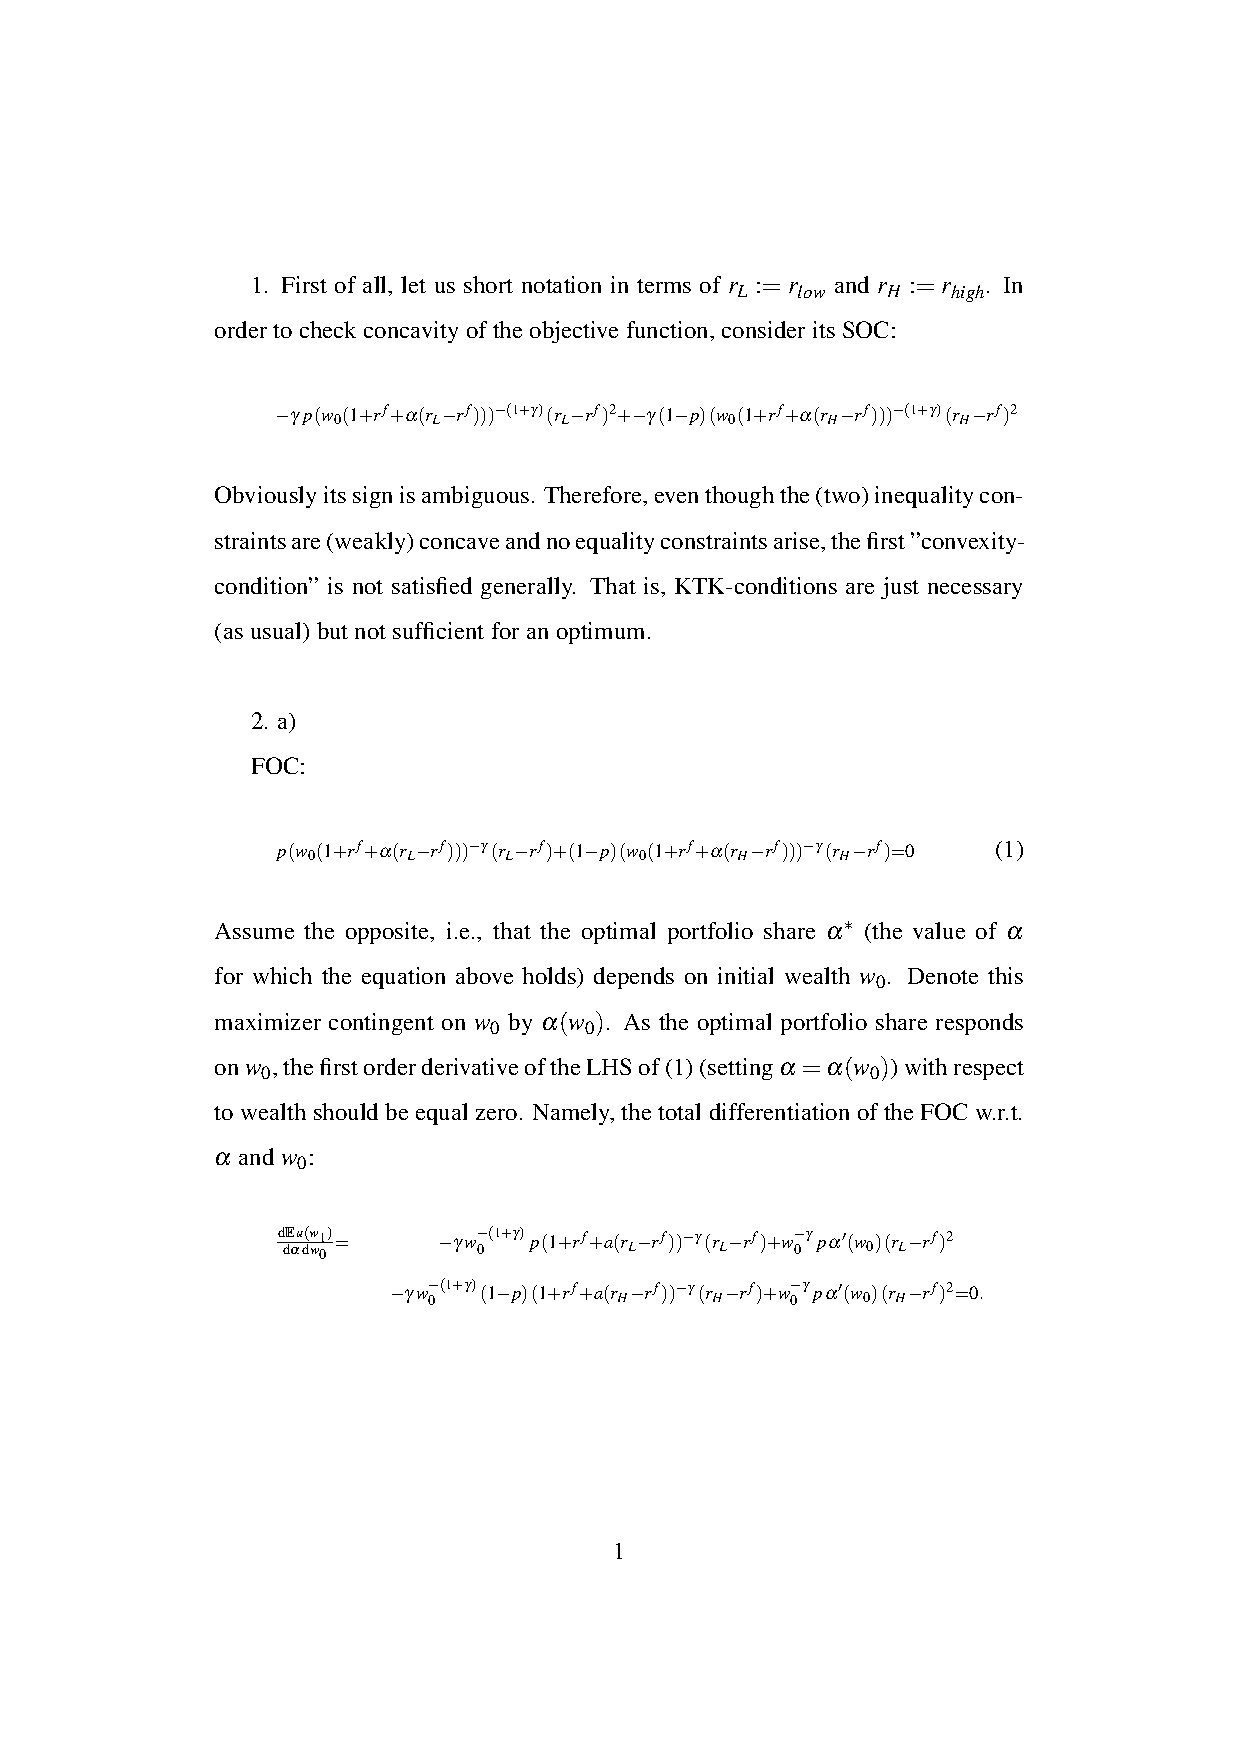
\includepdf[pages=-]{document.pdf} b) \newline

\lstinputlisting[style=Matlab-editor]{PS3Q5.m}
The fminbnd solution is at alpha=0.99993. The first fmincon solution, starting from the upper boundary is at alpha=0.99828. The second fmincon solution, starting from the lower boundary is at alpha=0.99767.
\\ \\
The two methods can yield different results because
\begin{enumerate} 
\item The way the constraints are defined differ. In fmincon, the can hold with equality, in fminbnd they have to hold with strict inequality. 
\item The way the algorithm searches for a minimum. fmincon starts at some point $x_0$ and moves along the $x$-axis while evaluating the function. fminbnd searches for a local minimum on the entire interval.
\end{enumerate}
\begin{figure}[H]
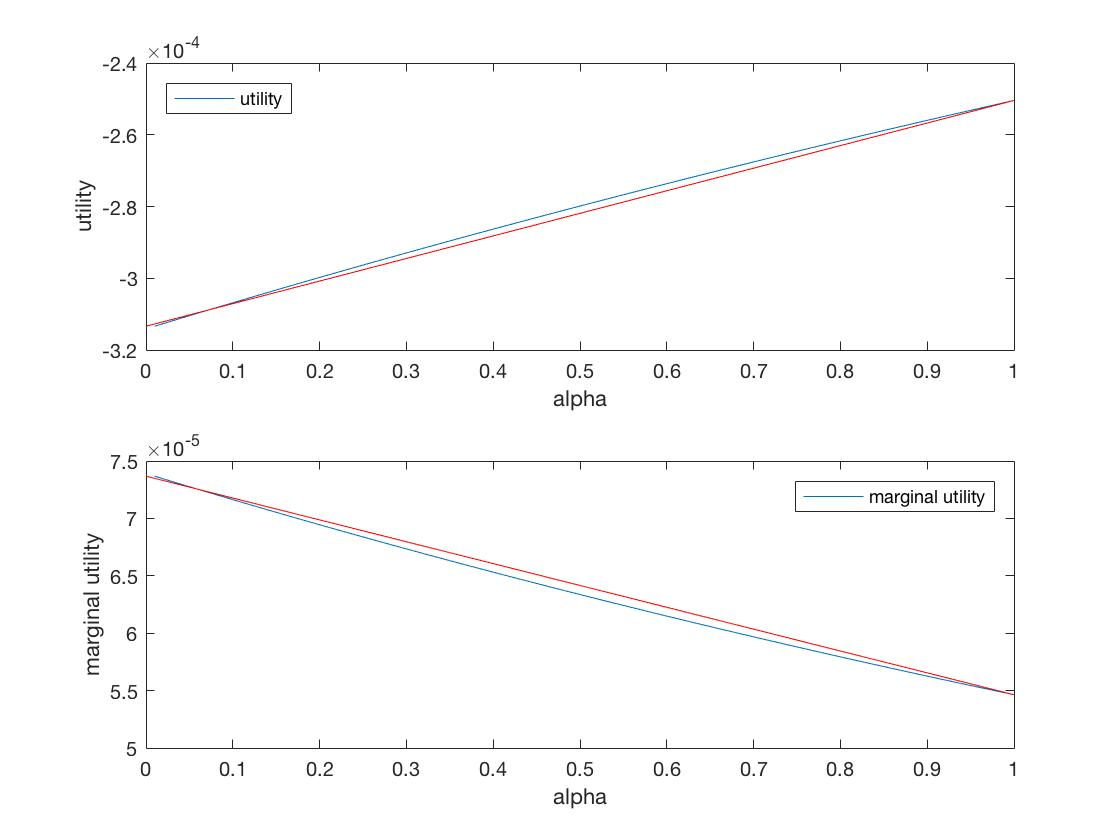
\includegraphics[width=\textwidth,height=\textheight,keepaspectratio, center]{PS3Q5Sub3bPlot.jpg} 
\caption{Illustration of the utility and marginal utility, depending on $\alpha$. \newline (The red line is a reference line with linear slope)}
\end{figure}
Comment: After running the algorithm for the first two times, the solutions produced by fmincon were = 1. The difference between the results from the two algorithms was then easily explainable by the difference in the interval constrains mentioned above ( $lb \leq \alpha \leq ub $ (fmincon) vs $ lb < \alpha < ub $ (fminbnd)). \\ \\
c) \\ \\
Part two of this question resulted in $\alpha = 2.73308$. However, the solution in part three was bounded on the upside at $\overline{\alpha} = 1$. The solution, derived numerically, resulted in $\alpha$ close to one (and one the first tries with fmincon resulted in $\alpha  = 1$, exactly the boundary). If one runs the maximization without the upper constrain, the argmax increases with the starting point (for fmincon (that the solution does not converge to infinity can be explained as the differences in function value lie below machine precision which results in a maximum being reported)). This implies that the household would like to borrow at the risk free rate (negative $\alpha^f$) to invest more in stocks to increase his expected portfolio return. \\ Since $\phi =  1- \gamma$ and $\phi =  -3$, it can be implied that $\gamma =  4$. Thus, the agent is risk averse. However, one would expect a risk averse agent not to borrow to invest into the risky asset. \\  
Looking at the utility function with the parameters specified in the question, $u(w_1)=\frac{\left(\frac{1}{w_1^3}\right )}{-3}$, it becomes obvious that with increasing wealth, the utility moves closer to zero from below as wealth increases. Since the probability to receive a high interest rate is nine times as large as the probability to receive a low interest rate, the expected return from the risky asset is much larger than the return of the safe asset. \\ Since the maximization problem can be rewritten as
\begin{align}
\max_\alpha \underbrace{ \frac{1}{\phi}}_{<0} \left( \underbrace{ w_0 \left(1+r^f + \alpha  \left(E [ r]- r^f\right) \right)}_{>0} \right) \underbrace{^\phi}_{<0}
\end{align}
which explains that $\alpha$ exceeds $1$ since there is no more uncertainty in the model. \end{document}